\chapter{Background}\label{ch:Background}

\section{Neutrinos}

The neutrino is a fundemental particle first proposed by Wolfgang Pauli \cite{nu_proposition}, and then later discovered in 1956 using the byproducts of $\beta^{-}$ decay \cite{aneut} in the form of the electron neutrino. As research continued into the elusive neutrino, another flavour of neutrino was discovered in 1962 called the muon neutrino ($\nu_{\mu}$) \cite{m_nu} and eventually the final flavour of the tau neutrino ($\nu_\tau$) \cite{t_nu}. 

\subsection{Oscillations}\label{subsec:osc}

Alongside the discovery of the neutrino and their flavours, another problem arose in the field of neutrino physics: the solar neutrino problem \cite{lowe_nu}. During the 1960's, an experiment was proposed by John Bahcall and Ray Davis to measure the solar neutrino flux, referred to as the Homestake experiment \cite{davis, bahcall}. This tank was filled with cleaning fluid which used $^{37}$Cl as the active agent in detection. It was built underground to avoid cosmic backgrounds, and used the reaction\cite{davis, bahcall}
\begin{equation}\label{eq:cl}
  \nu_{e} + ^{37}\text{Cl} \to e^{-} + ^{37}\text{Ar}
\end{equation}
to measure the expected solar neutrino flux from the sun. 

Solar neutrinos originate from nuclear processes that occur in the sun, mainly from the $pp$ chain and the CNO cycle. The $pp$ chain is described by the following reactions,
\begin{align}
  p + p \to & \, d + e^{+} + \nu_{e}\, ,  &  p + e^{-} + p \to & \, d + \nu_{e}\, , \\
  ^{3}\text{He} + p \to & \, ^{4}\text{He} + e^{+} + \nu_{e}\, ,  &  ^{7}\text{Be} + e^{-} \to & \, ^{7}\text{Li} + \nu_{e}(+\gamma)\, , \\
  ^{8}\text{B} \to & \, ^{8}\text{Be}^{*} + e^{+} + \nu_{e}\, ,
\end{align}
while the CNO cycle is described by
\begin{align}
  ^{13}\text{N} \to & \, ^{13}\text{C} + e^{+} + \nu_{e} \, ,  &   ^{15}\text{O} \to &\, ^{15}\text{N} + e^{+} + \nu_{e}\, ,\\
  ^{17}\text{F} \to & \, ^{17}\text{O} + e^{+} + \nu_{e} \, , 
\end{align}
and can be detected in experiments on Earth \cite{solar_nu,pdg}. It is easy to see that through these processes the internal processes of the sun produce primarily electron neutrinos. Depending on the energy and process producing the neutrino, we can expect to detect this particlar flavour of neutrino in experiments like the Homestake experiment. In particular, using the predicted distribution of the internal electron density of the Sun and a spectrum of the produced electron neutrinos, one could predict the expected flux of solar electron neutrinos \cite{solar_nu}. Using these previous processes, one would expect the flux of solar neutrinos to be purely electron flavoured yet it was found that the measured flux of neutrinos was consistently around 30\% the theoretical amount \cite{davis, bahcall, solar_nu}, and hence was coined the solar neutrino problem.

Neutrino detectors continued to be constructed to research and understand these fundemental particles, such as Kamiokande--II \cite{kam,kamioka} and Super--Kamiokande \cite{superk} from the collaboration of Kamiokande \cite{kam} and the IMB \cite{imb} experiments. The Kamiokande--II detector was a water cherenkov experiment for detecting $^{8}$B solar neutrinos through the neutrino--electron scattering interaction
\begin{equation}\label{eq:ES}
  \nu_{e} + e^{-} \to \nu_{e} + e^{-}\, ,
\end{equation}
which yields information on the neutrino arrival time, the direction, and the energy spectrum \cite{kamioka}. This detector boasted 2140 tonnes of water viewed by an array of 20 inch diameter photomultiplier tubes. Collecting data for 450 days from January 1987, the experiment found results consistent with the Homestake $^{37}$Cl experiment. The IMB experiment had a similar setup with a 3.3--kiloton fiducial mass and 2084 eight inch photomultiplier tubes, but was used to observe atmospheric neutrinos (neutrinos produced from cosmic ray interactions in the atmosphere) \cite{imb}. Yet again, the experiment found that the observed rates were lower than the theoretical expected rates \cite{imb}. To improve on these results and confirm they weren't statistical anomolies, the Super--Kamiokande detector was built as a 50--kiloton detector with 11,146 50--cm diameter photomultiplier tubes \cite{kam}. This massive upgrade from Kamiokande--II meant reduced uncertainties, and after detecting 900 muon--like and 983 electron--like events, the ratio of muon to electron neutrinos was compared to the expected theoretical result which again showed a reduced flux from expected \cite{kam}. The fact that these missing neutrinos were consistent between atmospheric and solar neutrinos meant there was something deeper going on than initially thought.

Another class of solar neutrino detectors were those that used the Gallium chain
\begin{equation}\label{eq:gal}
  \nu_{e} + ^{71}\text{Ga} \to e^{-} + ^{71}\text{Ge}\, ,
\end{equation}
such as GALLEX \cite{gallex}. Regardless, the same issue persisted as there continued to be a distinct dissonance between the theoretical expectations of solar neutrinos and the observed experimental results. That was, until the Sudbury Neutrino Observatory (SNO) made a distinct change in their approach to solar neutrino detection compared to predecessors by using heavy water \cite{sno}. This allowed for the following interactions \cite{sno},
\begin{align}
  \nu_{e} + d & \to p + p + e^{-} \label{eq:deut_1} \\
  \nu_{l} + d & \to p + n + \nu_{l} \label{eq:deut_2}
\end{align}
where we have the Charged Current (CC) interaction in equation \ref{eq:deut_1}, the Neutral Current (NC) interaction in equation \ref{eq:deut_2} and the electron scattering interaction just like in equation \ref{eq:ES}. This meant that all flavours of neutrinos could be detected, and using it to detect solar neutrinos showed the theoretical flux originally predicted \cite{sno}.

This result had an astounding implication; the neutrinos were changing on their journey from the Sun \cite{sno}. In the Standard Model, all the neutrino flavours have masses that are identically zero, and this would mean that there is no possible way for the neutrinos to somehow change flavour on their journey to the detectors \cite{solar_nu}. Clearly there was a change in flavour, and thus the Standard Model must be incorrect about the masses of the neutrinos.

The classic demonstrative method to describe this is to consider the mixing of two neutrino flavours (like $\nu_{\mu}$ and $\nu_{e}$) \cite{solar_nu}. In analogy to quark flavour mixing \cite{pdg_ckm}, we know the mixing of the flavours occurs in the transformation from the mass to the flavour basis. This means that the translation between considering the mass of the traveling neutrino against the falvour is non-trivial, and generally changing between one to the other is a super-position of states. In particular, for two mass and flavour states one can find \cite{solar_nu},
\begin{equation}
  P(\nu_{e} \to \nu_{\mu}, ct) = \sin^{2}2\theta\sin^{2}\left(\frac{\pi ct}{L}\right)
\end{equation}
where $\theta$ is the mixing between the two flavour states, $L = \frac{4\pi E}{\Delta m^{2}}$ is the vacuum oscillation length, and $\Delta m^{2} = m_{2}^{2} - m_{1}^{2}$ is the difference between the two mass squared values. It is important to note that when we say $\Delta m^{2}$, these mass values are not the masses of the flavour states, but rather values associated with another basis in which neutrinos travel \cite{pdg_ckm}. Here it is easy enough to see that the oscillation probability vanishes if the masses are identical, and this naturally extends into the three flavour case. The vacuum oscillation length, $L$, is an important and useful quantity as it describes the distance a neutrino must travel before an oscillation is expected \cite{solar_nu}; this behaves like the period of oscillation as it amplifies the probability of mixing for particular distances. Experiments like the long--baseline neutrino oscillation experiment Tokai--to--Kamioka (T2K) attempt to use this length to probe the mixing angles of the three neutrino flavours. 

Similar to the CKM matrix for quark mixing \cite{pdg_ckm}, the Pontecorvo--Maki--Nakagawa--Sakata (PMNS) matrix \cite{pmns} gives a relation between the mass and flavour states:
\begin{equation}
  \begin{bmatrix}
    \nu_{e} \\
    \nu_{\mu} \\
    \nu_{\tau}
  \end{bmatrix}
  =
  U
  \begin{bmatrix}
    \nu_{1} \\
    \nu_{2} \\
    \nu_{3}
  \end{bmatrix}
  \, 
\end{equation}
and we see that
\begin{equation}
  U = 
  \begin{bmatrix}
    c_{12}c_{13} & s_{12}c_{13} & s_{13}e^{-i\delta_{\text{CP}}} \\
    -s_{12}c_{23}-c_{12}s_{23}s_{13}e^{i\delta_{\text{CP}}} & c_{12}c_{23} - s_{12}s_{23}s_{13}e^{i\delta_{\text{CP}}} & s_{23}c_{13} \\
    s_{12}s_{23}-c_{12}c_{23}s_{13}e^{i\delta_{\text{CP}}} & -c_{12}s_{23} - s_{12}c_{23}s_{13}e^{i\delta_{\text{CP}}} & c_{23}c_{13}
  \end{bmatrix}
  \begin{bmatrix}
    e^{i\eta_{1}} & 0 & 0 \\
    0 & e^{i\eta_{2}} & 0 \\
    0 & 0 & 1
  \end{bmatrix}
\end{equation}
where $s_{ij} = \sin\theta_{ij}$, $c_{ij}=\cos\theta_{ij}$, $\delta_{\text{CP}}$ is the Charge--Parity violation phase \cite{pmns}, and $\eta_{i}$ are the Majorana phases. If neutrinos are not their own anti--particles, or in other words are Dirac fermions, we can expect $\eta_{i} = 0$. If they are their own anti--particles, also knowns as Majorana, then the phases $\eta_{i}$ play a more imporant role \cite{pdg}. 

\subsection{Interactions}\label{subsec:int}

Neutrinos are neutral and interact only through the Weak interaction. The Weak interaction is a force that is mediated by the $W^{\pm}$ and $Z^{0}$ massive bosons, and is the force responsible for decays. The main vertices involved in neutrino interactions are shown in Figure \ref{fig:nvert}, where the interacting lepton corresponds with the interacting neutrino flavour. 

\begin{figure}
  \centering
  \begin{tikzpicture}[scale=3]
    % W Boson
    \draw [boson] (0,0) -- (0.5,0);
    \node [left] at (0,0) {$W^{\pm}$};
    % lepton
    \draw [middlearrow={latex}] (0.5,0) -- (1,0.5);
    \node [right] at (1,0.5) {$\ell$};
    % neutrino
    \draw [middlearrow={latex}] (1,-0.5) -- (0.5,0);
    \node [right] at (1,-0.5) {$\nu_{\ell}$};
  \end{tikzpicture}
  \hspace{2em}
  \begin{tikzpicture}[scale=3]
    % Z Boson
    \draw [boson] (0,0) -- (0.5,0);
    \node [left] at (0,0) {$Z^{0}$};
    % lepton
    \draw [middlearrow={latex}] (0.5,0) -- (1,0.5);
    \node [right] at (1,0.5) {$\nu_{\ell}$};
    % neutrino
    \draw [middlearrow={latex}] (1,-0.5) -- (0.5,0);
    \node [right] at (1,-0.5) {$\nu_{\ell}$};
  \end{tikzpicture}
  \caption{The Feynmann diagrams for the vertices that would be included in neutrino interactions using the charged $W^{\pm}$ boson on the left and the neutral $Z^{0}$ boson on the right.}
  \label{fig:nvert}
\end{figure}

All interaction involving neutrino production or detection utilize these vertices in some shape or form. We refer to interactions that use the $W^{\pm}$ boson as the Charged Current (CC) interaction \cite{currents}, and those that use the $Z^{0}$ boson as being Neutral Current (NC) interactions \cite{currents}.

It is natural to notice that these interactions require something to interact with, or in other words, the neutrinos must propagate through non--vacuum media and hit targets. We have up to this point only considered oscillations of neutrinos in vacuum, and another imporant aspect is to consider the effect interactions could have on these oscillations. In particular, it is noted that certain flavours of neutrinos can be more strongly influenced by media than others \cite{solar_nu,msw}. Electrons are much more prevalent in matter than the other two generations ($\mu,\,\tau$) and hence the electron neutrino ($\nu_{e}$) tends to experience a larger interaction than the other flavours \cite{solar_nu,msw}. This difference in coupling results in changes in the oscillation that is complex.

This phenomena comes to a head with the Mikheyev–Smirnov–Wolfenstein (MSW) effect. The mixing angle and oscillation length vary with the electron density in the medium which varies the rate at which these neutrinos mix \cite{solar_nu,msw}. In particular there is a resonance mixing angle (and hence resonence electron density) at which the mixing is maximized \cite{solar_nu,msw}. The electron density at the centre of the sun starts far above the resonance and ends below the resonance at the edge, hence the produced electron neutrinos experience this resonance oscillation along their path out of the solar center \cite{solar_nu,msw}. Neutrino oscillations are the reason for the solar neutrino problem, and the MSW effect is the catalyst \cite{solar_nu}.

\subsection{Solar Production}

As was discussed in subsection \ref{subsec:osc} and \ref{subsec:int}, neutrinos produced in the fusion process hold great historical significance, and in the attempt to resolve the solar neutrino problem we have come to better understand neutrinos and their processes. The leading reaction chain is the $pp$ chain \cite{pdg,solar_nu}, which is given by \cite{pdg}
\begin{equation}
  p + p \to d + e^{+} + \nu_{e} \, .
\end{equation}
All other chains that fall under the $pp$ chain follow a similar idea; through the charged current interaction, there is the production of an electron neutrino during the fusion of two reactants \cite{pdg}.

\subsection{Atmospheric Production}\label{subsec:atmos}
Another site where we can observe neutrino production is in the atmosphere \cite{atm_nu,pdg,volk_atm}. These neutrinos are primarly produced by the decay of pions and muons \cite{pdg},
\begin{align}
  \pi^{+} & \to \mu^{+} + \nu_{\mu}\, , \\
  \mu^{+} & \to e^{+} + \nu_{e} + \bar{\nu}_{\mu}
\end{align}
and the charge conjugate $\pi^{-}$ \cite{pdg}. The production of these decaying pions and muons is initiated by cosmic rays interacting with the nucleons in the atmosphere \cite{atm_nu,pdg,volk_atm}. Looking at the inciting interactions, a natural and useful ratio is 
\begin{equation}
  \frac{\nu_{\mu} + \bar{\nu}_{\mu}}{\nu_{e} + \bar{\nu}_{e}}
\end{equation}
of the number densities \cite{pdg}. It is also useful to note that atmospheric neutrinos can be both downward heading and upward heading, as they can travel through the earth. These two different directions will experience different travel lengths and can be used to probe neutrino oscillations \cite{pdg}. There have been studies done on the atmospheric neutrino flux with experiments across the globe \cite{pdg, volk_atm}.

\subsection{Geological Production}
Neutrinos can also be generated by the natural decay of rare elements in the Earths crust \cite{geo_nu}. In particular, the main source is of $\beta^{-}$ decays in elements like $^{238}$U, $^{232}$Th and $^{40}$K \cite{geo_nu}. Measuring the geo--neutrino flux holds interesting consequences in the geology and physics community, for example predictions of the radiogenic contributions by neutrino producing processes can be predicted \cite{geo_nu}.

\subsection{Reactor Production}
Production of neutrinos by $\beta^{-}$ decay also occurs in reactors \cite{re_nu}. The fission process involving $^{235}$U uses a chain reaction of neutron production to fuel more fissions \cite{re_nu}, and this neutron rich environment promotes the classic bound neutron decay,
\begin{equation}
  n \to p + e^{-} + \bar{\nu}_{e}\, .
\end{equation}
The benefit of using reactor neutrinos lies in the flavour purity; the production mechanism promotes the creation of electron anti--neutrinos \cite{re_nu}.

\subsection{Accelerator Production}
Accelerator neutrinos are produced by firing a beam of protons at a target to produce secondary mesons that decay and produce neutrinos \cite{acc_nu}. This process is similar to the atmospheric neutrino production process as the idea is similar: secondary mesons produced by high energy primaries that then decay and produce neutrinos. The benefit of this production method is they are generally produced in a collimated beam within some angular range due to the momentum based production \cite{acc_nu}. This effectively produces a neutrino beam that can then be used in later processing.

\subsection{Galactic Production}
Supernovas can produce high energy neutrinos that can travel thousands of years before reaching detectors on earth \cite{sup_nu}. These provide both unique insights into the universe, as they will leave a higher energy signature \cite{sup_nu} and the vast distance travelled allows for the neutrino to arrive at the earth in a mass eigenstate. The reason for arriving in the eigenstate occurs as a result of the large distance allowing for the competing mass states to decouple \cite{sup_nu}. 

Another proposed galactic source of high energy neutrinos are Active Galactic Nuclei (AGN) which are potentially the most powerful producers of radiation in the universe \cite{agn_nu}. AGNs are known for accelerating protons up to $10^{20} - 10^{21}$ eV, and provide a potential pathway for producing incredibly high energy neutrinos \cite{agn_nu}.

\section{Detection Techniques}

With a plethora of neutrino sources, some of which have been discussed, the method of detection becomes increasingly important. For the purposes of this text, we only consider a couple of techniques that are of interest. To begin, we can consider the GALLAX type experiments that use the chain identified in equation \ref{eq:gal}.

\subsection{Germanium Detectors}

These are blind to the other flavours of neutrinos, as was already discussed, but they did motivate using Germanium as a potential neutrino detection method. In particular there are propositions that these detectors may provide $\mathcal{O}(1 \text{kg})$ mass, $\mathcal{O}(100 \text{eV})$ threshold and $\mathcal{O}(1 \text{kg}^{-1}\text{keV}^{-1}\text{day}^{-1})$ background experiments \cite{som_germ}. In particular, detectors like these could be sensitive to low energy solar neutrinos through neutrino--nucleus elastic scattering \cite{germ_low} where the lower energy neutrinos can have an amplified signal through internal charge amplification \cite{germ_low}.

\subsection{Calorimeters}

Another class of neutrino detectors use calorimeters as a method of detecting energy deposits from secondaries in neutrino producing processes \cite{minos,ical}. These signals can then be used to reconstruct the neutrino flavour and energies \cite{minos,ical}. Two examples of such detectors are MINOS \cite{minos} and ICAL \cite{ical}. The former uses a proton beam on a graphite target to produce showers of hadrons that are then focused by two magnetic horns in a calorimeter \cite{minos}. These hadron showers consist of pions and, at higher energies, kaons which produce our neutrinos in their decays \cite{minos}. ICAL is a calorimeter array located at the India--based Neutrino Observatory \cite{ical} that can use external sources of neutrinos (atmospheric) to probe the mixing angles \cite{ical}. In particular ICAL can be particularly sensitive between neutrinos and anti--neutrinos \cite{ical}.

\subsection{Vavilov--Cherenkov}

Now that we have an appreciation for some novel techniques in detecting neutrinos, we discuss one that is of particular interest for the purposes of this thesis: Vavilov--Cherenkov (VC) Radiation. VC Radiation was discovered in 1934 by Vavilov \cite{vav_og} and Cherenkov \cite{cher_og} and then later in 1937 explained by Tamm and Frank \cite{tamm}. In essence, VC Radiation is the emission of electromagnetic radiation due to a charged particle traveling in a medium at a velocity, $v$, that exceeds the phase velocity, $v_{p}$, of light in that medium \cite{ginz}. In particular, if we suppose the velocity of light in vacuum is $c$, then VC Radiation will occur if
\begin{equation}
  v > v_{p} = \frac{c}{n(\omega)}\, ,
\end{equation}
where $n(\omega)$ is the frequency dependent index of refraction in that medium \cite{ginz}. In particular, if the light is emitted along a wave--vector $\vec{k}$ from a charged particle traveling with velocity $\vec{v}$, then the angle between the two vectors is $\theta_{0}$ and can be described by
\begin{equation}\label{fig:cher_angle}
  \cos\theta_{0} = \frac{c}{n(\omega)\cdot v}\,
\end{equation}
where $v = |\vec{v}|$ \cite{ginz}. Due to the electromagnetic radiation wavefront being a result of spherical emissions \cite{ginz}, the process is very similar to that of the acoustic sonic boom for macroscopic objects \cite{ginz} which serves as an excellent analogy.

This particular form of radiation is incredibly useful for neutrino detection. We can use the secondary leptons produced in CC interactions, like those in Figure \ref{fig:nvert}, to produce VC Radiation that can be detected by ultra sensitive photon detectors. 

\section{Neutrino Telescopes}

Generally one considers only telescopes as those that utilise the visible part of the electromagnetic spectrum, and in general this is true, but as technology has advanced we have found that using even other wavelengths of light has resulted in different information to be gained from the imaging of the universe. This idea can be extended to include other sources or even particles to image with, like the neutrino. Due to the weakly interacting nature of the neutrino it can travel great distances before interacting and can provide direct sources where cosmic rays may be ambigious about their source. Neutrino telecopes use exactly this principle to reconstruct neutrinos from cosmic sources with the potential to image the sky one day in an entirely different lens.

The DUMAND experiment \cite{dumand} was the first to propose the use of large photomultiplier tubes in deep ocean to detect high energy neutrinos. Though it was never brought to fruition, it was the first of its kind and paved the way for future VC Radiation based neutrino telescopes such as Baikal \cite{baikal}, AMANDA \cite{amanda}, ANTARES \cite{antares}, and IceCube \cite{icecube}. We will discuss a few of these that are relevant. 

\subsection{IceCube}

The IceCube Neutrino Observatory is a cubic--kilometer neutrino detector built in the Antarctic ice \cite{icecube}. Its primary scientific goal was the detection and characterization of astrophysical neutrinos along with their sources \cite{icecube}, but also has many other scientific goals including indirect detection of dark matter, exotic particle searches, neutrino oscillations, and supernova neutrinos \cite{icecube}.

Neutrino detection occurs through VC Radiation of charged particles from neutrino interactions traveling through the ice \cite{icecube}. IceCube has the advantage of having a very large volume coverage in order to compensate for the small neutrino cross--section and low astrophysical sources flux \cite{icecube}. The detection is done through the Digital Optical Module (DOM) consisting of $10^{\prime\prime}$ Photo--Multiplier Tubes (PMTs) which are sensitive to the VC photons \cite{icecube}. The full array is has 5160 DOMs on 86 vertical strings where each string consists of 60 DOMs \cite{icecube}. The array sits between 1450 meters and 2450 meters below the surface of the ice \cite{icecube}.

The detection medium of ice is novel in the neutrino telescope field and offers both advantages and disadvantages over water \cite{icecube_rad}. Ice that has been undisturbed, like that in the Antarctic, offers pure conditions and is stationary when compared with the flow of most large bodies of water \cite{icecube_rad}. However, equipment that is used in the ice is not recoverable \cite{icecube_rad} and hence difficult to repair. Moreover, ice offers a shorter scattering length than one would expect in water \cite{icecube_rad} and due to the ice being layered this effect is layer dependent and was studied in detail to build reference tables \cite{icecube_rad}.

IceCube has been successful in its original physics goal \cite{icecube} and in 2017 detected a high energy neutrino estimated to have an energy of 290 TeV \cite{icecube_nat}. This was coincident in direction and time with a gamma--ray flare from blazar TXS 0506+056 \cite{icecube_nat}. Studying previously collected data in search for more high energy events of the same caliber from the same direction supported the claim that blazars can be a source of high energy neutrinos \cite{icecube_nat}. IceCube is continuing to collect data and explore more of its physics goals.

\subsection{ANTARES}

The ANTARES neutrino telescope is the first operational neutrino telescope in the Mediterranean Sea \cite{antares} adopting heavily from DUMAND \cite{dumand} and Baikal \cite{baikal}. Similar to other neutrino telescopes, the main method of neutrino detection arises from VC Radiation from secondary leptons produced in neutrino interactions \cite{antares}. The array is composed of 12 mooring lines equipped with 25 Optical Modules (OMs) that contain PMTs for a total of 885 OMs (the $12^{\text{th}}$ line has a different number of OMs) \cite{antares}.

Compared to the experiments that use ice, like Icecube \cite{icecube, icecube_nat, icecube_rad} and AMANDA \cite{amanda}, ANTARES uses ocean water as the medium of VC Radiation from high energy neutrino induced leptons \cite{antares}. The benefit over ice is that the attenuation/scattering length is longer, and the lack of layering reduces the reconstruction difficulties \cite{antares, icecube_rad}. The difficulties are that the water shifts, and hence can both rotate the detectors slightly and move their relative positions \cite{antares, icecube_rad}. To account for this shifting, ANTARES uses a High Frequency Long Base Line (HFLBL) acoustic system providing 3D positions of hydrophones positioned along the mooring lines \cite{antares}. To account for the tilting, each OM is given a set of tiltmeter--compass sensors giving the local tilt angles of each OM structure \cite{antares}. Moreover, there are backgrounds from $^{40}$K decay and bioluminesence to consider \cite{icecube_rad}.

ANTARES was finished construction in 2008 and has been collecting data since \cite{antares}. They have achieved their design goals and are able to achieve a positional accuracy better than 20 cm for each OM with the expected time resolution of 1 ns \cite{antares}. This experiment shows the feasibility of water based neutrino telescopes and opens the doors for future ocean neutrino telescopes. 

\subsection{Baikal}

Another large influence in the neutrino telescope experimental community is the neutrino telescope deployed in lake Baikal \cite{baikal}. First constructed in 1998 \cite{baikal}, this historic neutrino telescope has been since upgraded with more detectors and recently has been continuing upgrades to become the Baikal--GVD (Baikal Gigaton Volume Detector) \cite{baikal_gvd}. The lake itself is covered in a thick layer of ice during the winter and allows for construction using the temporary platform \cite{baikal}.

The Baikal--GVD neutrino telescope makes use of the VC radiation from high energy neutrino induced leptons to make measurements, as is expected of a detector located in a water medium \cite{baikal, baikal_gvd}. Select data has been processed and analyzed as data taking continues through additions of the pieces that will eventually make up the full Baikal--GVD telescope \cite{baikal_gvd}, where the physics goals were originally to provide insight into both neutrinos and the cosmic sources that produce them \cite{baikal}.

\begin{figure}[H]
  \centering
  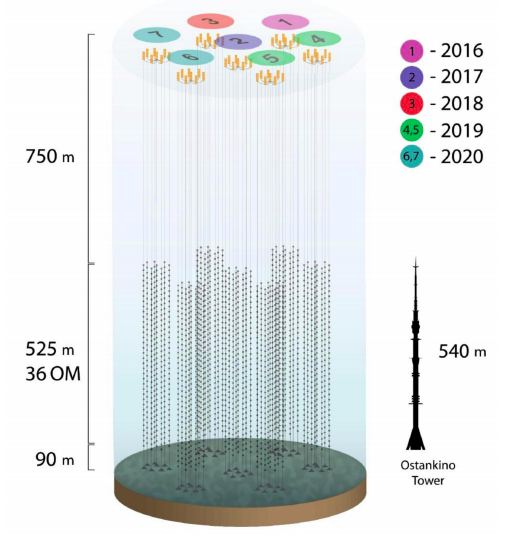
\includegraphics[width=12cm]{./Figures/baikal-gvd.png}
  \caption{A figure showcasing the Baikal--GVD telescope once fully complete, highlighting the timescales for when each section is scheduled for construction \cite{baikal_gvd2020}.}
  \label{fig:baikal}
\end{figure}

Baikal-GVD continues construction and set to be complete soon \cite{baikal_gvd2020} following which it will collect data and release results.

\subsection{KM3NeT}

Similar to ANTARES, the Cubic Kilometer Neutrino Telescope (KM3NeT) is a neutrino telescope located in the Mediterranean \cite{km3net}, and hence functions in a similar manner by utilizing VC radiation from high energy neutrino induced leptons \cite{km3net}. The largest improvement from ANTARES is that KM3NET is massive in scale, and plans to overshadow the size of even IceCube with it's full detector \cite{km3net}. Moreover, the location of the detector in the Mediterranean complements the coverage provided by IceCube and can support a Global Neutrino Network coverage \cite{km3net}.

The detector will consist of three deep--sea sites located off--shore from Toulon (France), Capo Passero (Italy) and Pylos (Greece) \cite{km3net}. Each site is planned to have 115 strings, 18 optical modules per string with each optical module containing 31 PMTs. Two of the sites will be in support of and further exploration of astroparticle goals (detection of high energy neutrinos from galactic sources) and are referred to as ARCA (Astroparticle Research with Cosmics in the Abyss). The remaining site will be primarily for oscillation measurements, and is referred to as ORCA (Oscillation Research with Cosmics in the AByss). These sites are highlighted in Figure \ref{fig:km3net}, alongside the collaborating cities. 

\begin{figure}[H]
  \centering
  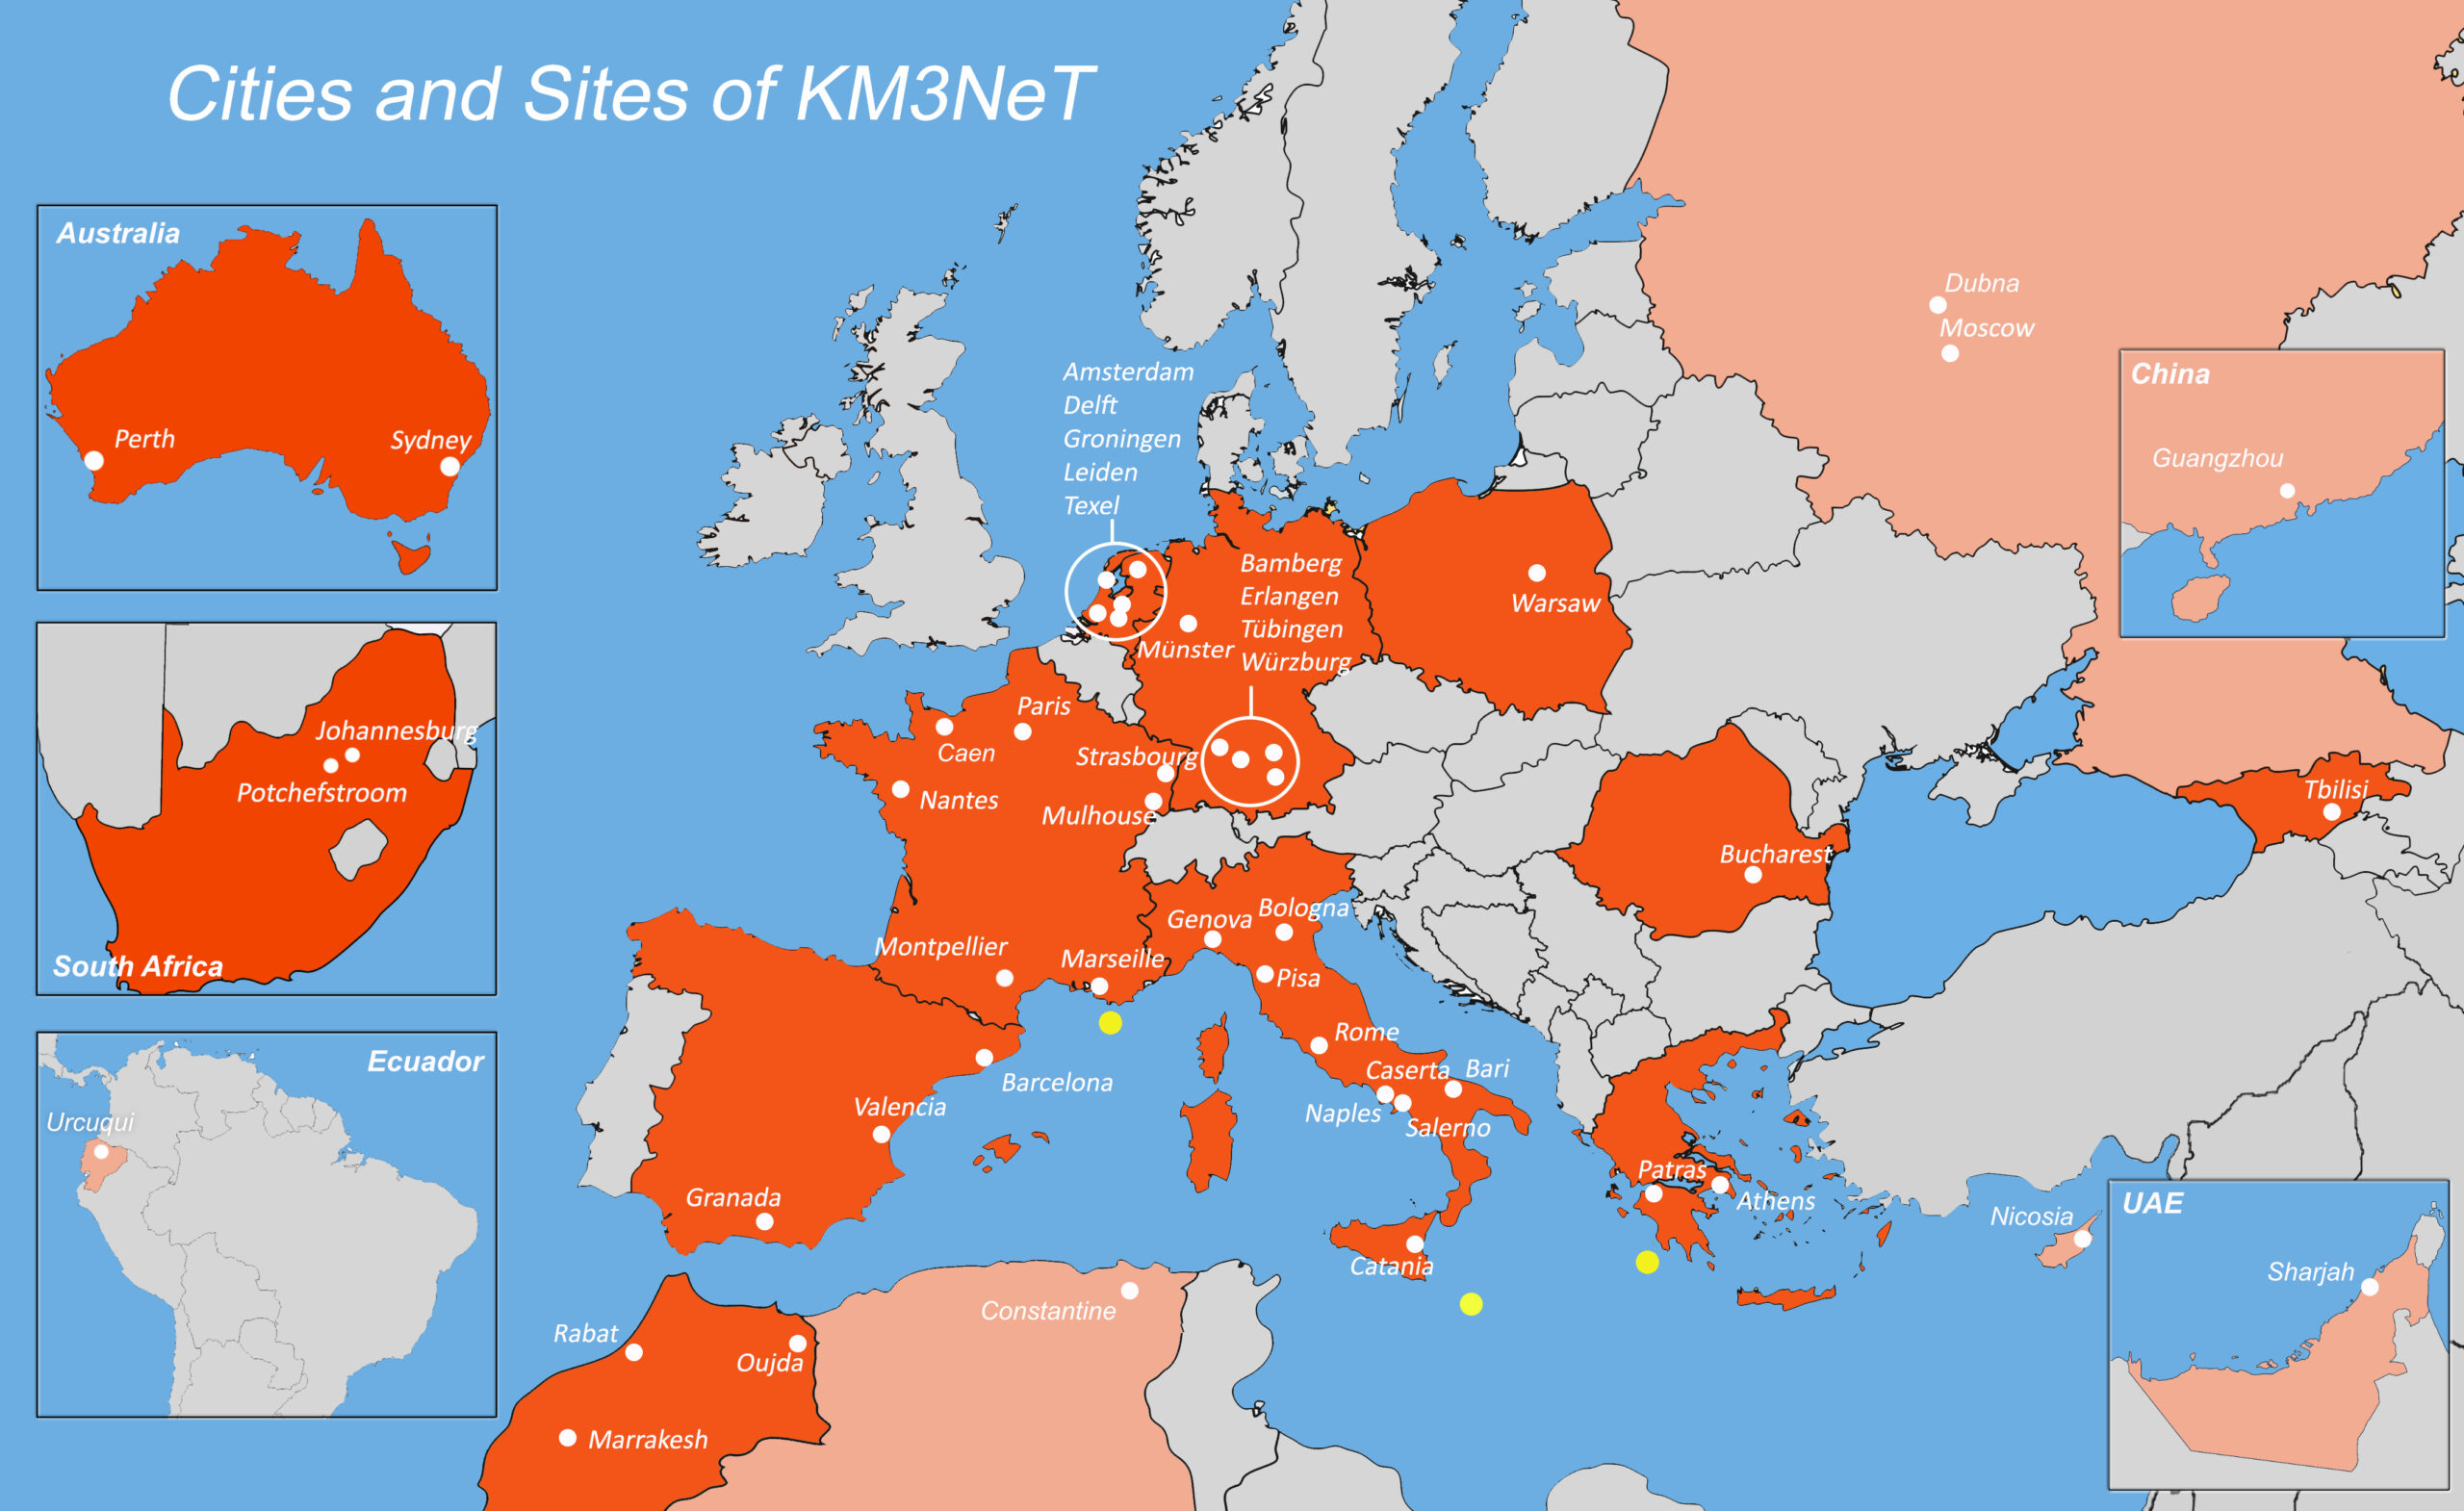
\includegraphics[width=12cm]{./Figures/KM3NeT.jpg}
  \caption{A figure showcasing the KM3Net collaboration group locations and the locations of the three cites for construction marked in yellow. Original image can be found on the KM3Net homepage \cite{km3net_web}.}
  \label{fig:km3net}
\end{figure}

KM3NeT plans to have completed all construction within the next decade and continue data collection for atleast a decade following completion of construction \cite{km3net}.



